\documentclass{beamer}
\usepackage{beamerthemeshadow}
\usepackage{graphicx}
\usepackage{color}
\usepackage[utf8]{inputenc}
\usepackage{hyperref}
\usepackage[flushleft]{threeparttable}
\usepackage[english,serbian]{babel}
\definecolor{beamer@darkred}{rgb}{0.85,0.1,0.1}
\setbeamercolor{structure}{fg=beamer@darkred}

\title{Tehničko i naučno pisanje}
\subtitle{VAR tehnologija}
\author{Luka Šešelja, Ognjen Arsenijević, Ognjen Radivojević}
\institute{Matematički fakultet\\Univerzitet u Beogradu}
\date{\footnotesize{Beograd, 2022.}}

\begin{document}
\begin{frame}
\titlepage
\end{frame}

\begin{frame}[fragile]{Literatura}
    \begin{itemize}
        \item \em{Video assistant referee}. (2022, December 16). In Wikipedia. 
        \item Gidget Alikpala. \em{Qatar 2022 World Cup: What is the VAR and when is it used?} (Diario AS, 2022, December 16).
        \item Jochim Spitz, Johan Wagemans, Daniel Memmert, A. Mark Williams, Werner F. Helsen. \emph{Video assistant referees (VAR): The impact of technology on decision making in association football referees}. Routledge, 2021. 
        \item  Nevill, Alan and Balmer, Nigel and Williams, Andrew. \emph{The Influence of Crowd Noise and Experience upon Refereeing Decisions in Football}. Psychology of Sport and Exercise, 2002.
        \item Henning Plessner, Tilmann Betsch. \emph{Sequential Effects in Important Referee Decisions:The Case of Penalties in Soccer}. Human Kinetics Publishers, Inc, 2001.
    \end{itemize}
\end{frame}

\begin{frame}
  \frametitle{Pregled}
  \tableofcontents
\end{frame}

\section{Uvod}

\begin{frame}
  \frametitle{VAR tehnologija}
  \begin{itemize}
    \item Šta je VAR tehnologija?
    \item Prednosti VAR-a
    \item Kontroverznost VAR-a
  \end{itemize}
\end{frame}

\begin{frame}
  \frametitle{Istorija}
  \begin{itemize}
    \item Prva ideja o upotrebi video tehnologije u fudbalu
    \item Prvi test uživo
    \item Monitor pored terena
    \item Zvanična implementacija VAR-a u pravila fudbala
    \item VAR danas
  \end{itemize}
\end{frame}

\section{Primena VAR tehnlogije u praksi}

\begin{frame}
  \frametitle{Slucajevi u kojima se koristi VAR tehnologija}
  \begin{itemize}
    \item Gola ili prekršaja koji dovodi do gola.
    \item Penala ili prekršaja koji dovodi do penala.
    \item Dodele direktnog crvenog kartona.
    \item Greške pri identifikovanju igrača.
  \end{itemize}
\end{frame}

\begin{frame}
  \frametitle{Podešavanje kamera}
    \begin{figure}[h!]
    \begin{center}
    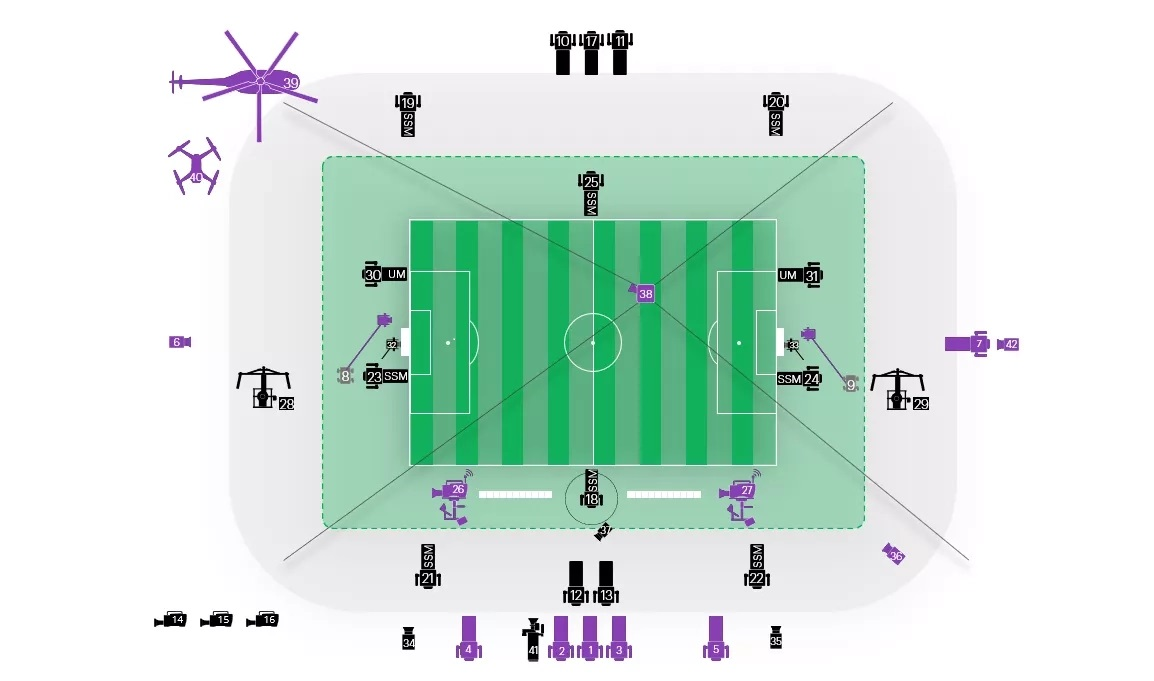
\includegraphics[scale=0.30]{Var sistem.jpeg}
    \end{center}
    \caption{Raspored kamera na terenu u okviru VAR sistema}
    \label{fig:kamere}
\end{figure}
\end{frame}
\begin{frame}
  \frametitle{VAR tim}
  Var tim se sastoji od:
    \begin{itemize}
    
        \item VAR sudije
        \item Prvog asistenta VAR sudije (AVAR1)
        \item Drugog asistenta VAR sudije (AVAR2)
        \item Trećeg asistenta VAR sudije(AVAR3)
        \item Sudijske oblasti za pregled (eng. Referee review area (RRA))
    \end{itemize}
    \begin{figure}[h!]
    \begin{center}
    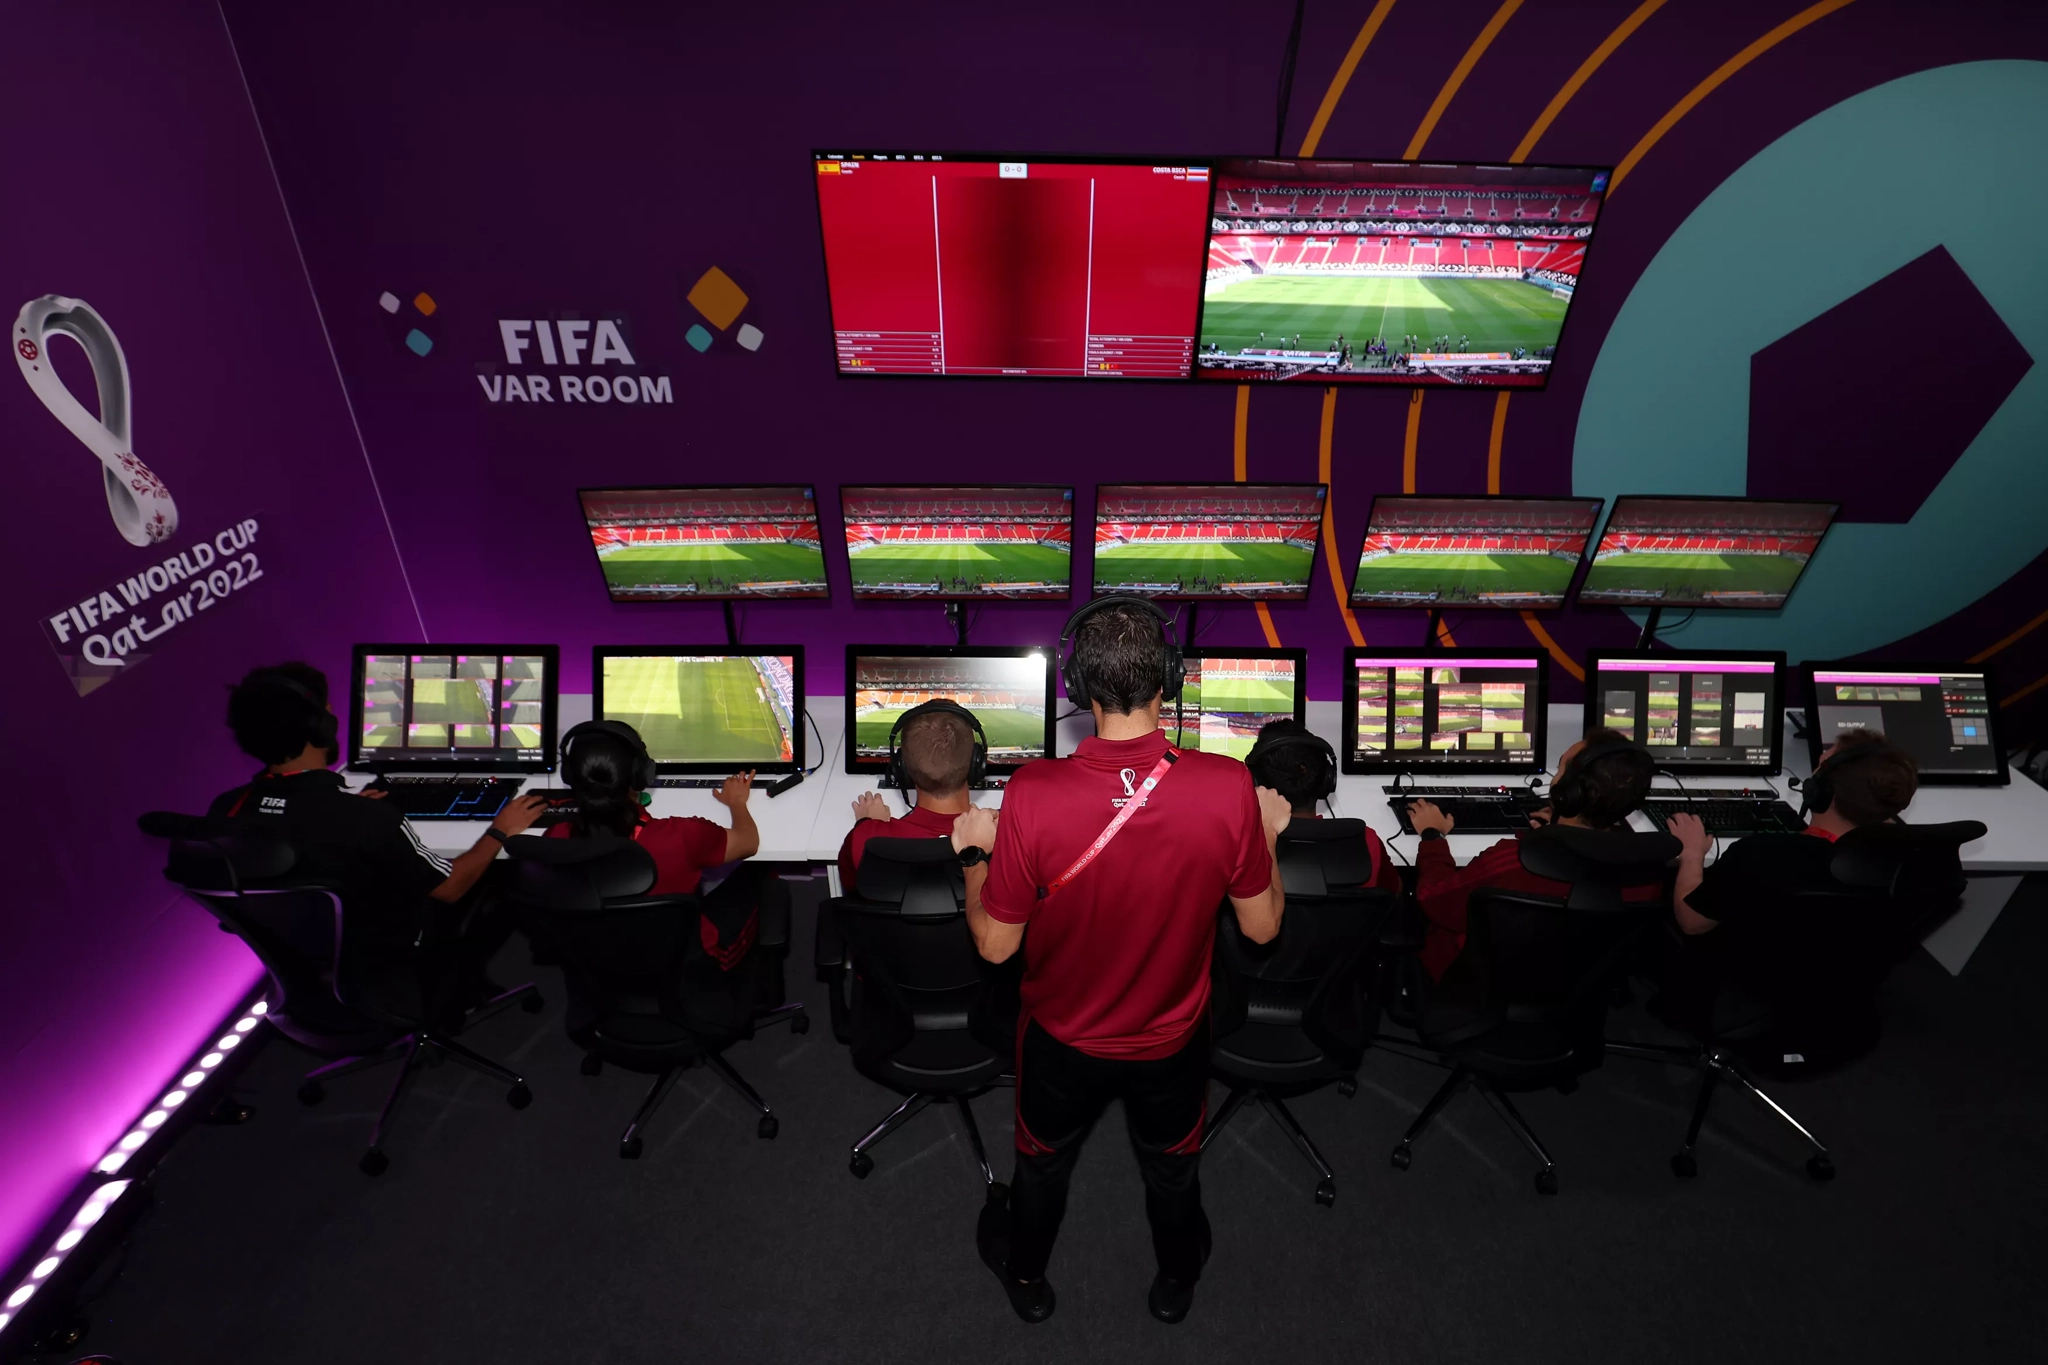
\includegraphics[scale=0.10]{var.png}
    \end{center}
    \caption{Članovi VAR tima}
    \label{fig:vartim}
\end{figure}
\end{frame}


\section{Preciznost provera}

\begin{frame}
  \frametitle{Preciznost i trajanje provera}
  \begin{itemize}
    \item  Ispravnost sudijske odluke
    \item  Trajanje provere i pregleda
    \item  Statistička analiza
  \end{itemize}
\end{frame}

\begin{frame}
  \frametitle{Preciznost odluka (\%)}
  \begin{itemize}
    \item  Tačnost i broj provera
    \item  Siva zona i sudijske odluke
    \item  Tipovi indidenata
  \end{itemize}
\end{frame}

\section{Zaključak}

\begin{frame}
  \frametitle{Zaključak}
  \begin{itemize}
    \item  Skinut pritisak sa sudija na terenu
    \item  Šta je VAR doneo dobro
    \item  Šta je VAR doneo loše
  \end{itemize}
\end{frame}


\end{document}
